\documentclass[usenatbib,usegraphicx,letterpaper]{mn2e}
\usepackage[totalwidth=480pt,totalheight=680pt]{geometry}

\usepackage{lmodern}

\usepackage{amsmath}
\usepackage{amstext}
\usepackage{amssymb}
\usepackage{yfonts}

\usepackage{epsfig}
\usepackage{graphicx}
\usepackage{color}

\usepackage[lowtilde]{url}
\usepackage{hyperref}

\bibliographystyle{mn2e}

%-------- journals
\newcommand{\araa}{ARAA~}
\newcommand{\apj}{ApJ~}
\newcommand{\apjl}{ApJL~}
\newcommand{\apjs}{ApJS~}
\newcommand{\mnras}{MNRAS~}
\newcommand{\nat}{Nature~}
\newcommand{\physrep}{Phys. Rep.~}
\newcommand{\aj}{AJ~}
\newcommand{\pasp}{ASP~}

%%%% Misc %%%
\newcommand{\beq}{\begin{equation}}
\newcommand{\eeq}{\end{equation}}
\newcommand{\beqray}{\begin{eqnarray}}
\newcommand{\eeqray}{\end{eqnarray}}

\newcommand{\ben}{\begin{enumerate}}
\newcommand{\een}{\end{enumerate}}
\newcommand{\bit}{\begin{itemize}}
\newcommand{\eit}{\end{itemize}}

%%%%%%%%  galaxy properties  %%%%%%%%
\newcommand{\rhalf}{R_{1/2}}
\newcommand{\rhalfdisk}{R_{1/2}^{\rm disk}}
\newcommand{\rhalfbulge}{R_{1/2}^{\rm bulge}}
\newcommand{\adisk}{A_{\rm disk}}
\newcommand{\abulge}{A_{\rm bulge}}
\newcommand{\alphadisk}{\alpha_{\rm disk}}
\newcommand{\alphabulge}{\alpha_{\rm bulge}}
\newcommand{\sigmarhalf}{\sigma_{\rm R_{1/2}}}
\newcommand{\bt}{{\rm B/T}}
\newcommand{\mstar}{M_{\ast}}
\newcommand{\ssfr}{{\rm sSFR}}
\newcommand{\sfr}{{\rm SFR}}

%%%%%%%%  halo properties  %%%%%%%%
\newcommand{\halospin}{\lambda_{\rm halo}}
\newcommand{\mvir}{M_{\rm vir}}
\newcommand{\macc}{M_{\rm acc}}
\newcommand{\mpeak}{M_{\rm peak}}
\newcommand{\zpeak}{z_{M_{\rm peak}}}
\newcommand{\mhalo}{M_{\rm halo}}
\newcommand{\mhost}{M_{\rm host}}
\newcommand{\rvir}{R_{\rm vir}}
\newcommand{\rmpeak}{R_{\rm M_{peak}}}
\newcommand{\vmaxmpeak}{V_{\rm peak}}
\newcommand{\vmax}{V_{\rm max}}
\newcommand{\rspeak}{{R_{\rm s,}}_{\rm M_{peak}}}


%%%%%%%%  cosmology  %%%%%%%%
\newcommand{\lcdm}{\Lambda{\rm CDM}}

%%%%%%%%  observations  %%%%%%%%
\newcommand{\rproj}{r_{\rm p}}
\newcommand{\wproj}{w_{\rm p}}
\newcommand{\wplarge}{w_{\rm p}^{\rm large}}
\newcommand{\wpsmall}{w_{\rm p}^{\rm small}}
\newcommand{\wpall}{w_{\rm p}^{\rm all}}

\newcommand{\mean}[2]{\langle{#1}\vert{#2}\rangle}
\newcommand{\median}[2]{\langle{#1}\vert{#2}\rangle_{\rm median}}

%%%%%%%%  units  %%%%%%%%
\newcommand{\kpc}{{\rm kpc}}
\newcommand{\mpc}{{\rm Mpc}}
\newcommand{\msun}{M_\odot}
\newcommand{\kms}{{\rm km/s}}

%%%%%%%%%%%%%%%%%%%%%%%%%%%%%%%%
%%%%%%%%%%%%%%%%%%%%%%%%%%%%%%%%


\usepackage{epsfig}  \usepackage{graphicx}   \usepackage{rotating}

\begin{document}

\title[The Relative Sizes of Centrals and Satellites]
{Clustering Constraints on the Relative Sizes of Central and Satellite Galaxies}


\author[Hearin, Behroozi, Kravtsov \& Moster]{
Andrew Hearin$^{1}$, Peter Behroozi$^{2}$, Andrey Kravtsov$^{3}$, Benjamin Moster$^{4}$\\
$^{1}$Argonne National Laboratory, Argonne, IL, USA 60439, USA\\
$^{2}$Department of Physics, University of Arizona, 1118 E 4th St, Tucson, AZ 85721 USA\\
$^{3}$Department of Astronomy \& Astrophysics, and Kavli Institute for Cosmological Physics, University of Chicago, Chicago IL 60637\\
$^{4}$Universit{\"a}ts-Sternwarte, Ludwig-Maximilians-Universit{\"a}t M{\"u}nchen, Scheinerstr. 1, 81679 M{\"u}nchen, Germany
}

\maketitle

\begin{abstract}
We place empirical constraints on the connection between dark matter halos and galaxy half-light radii, $\rhalf.$ Low-redshift SDSS measurements show that smaller galaxies cluster much more strongly than larger galaxies at fixed stellar mass. Using {\tt Halotools} to forward model the observations, we find that the clustering signal generically requires satellite galaxies to be smaller than central galaxies of the same halo mass. We present a simple empirical model consistent with the clustering results, in which galaxy size is proportional to halo virial radius at the time of peak halo mass. We use this model to predict how galaxy lensing, $\Delta\Sigma,$ should depend on $\rhalf$ for $\mstar-$complete samples. Other simple empirical models fail the clustering test, such as models in which galaxy size is related to stellar mass alone; these failures persist even when accounting for possible effects from satellite stripping and orphan galaxies. Our results suggest that the relative size of centrals and satellites is predetermined at the time of satellite infall, and that a remarkably simple galaxy--halo scaling relation emerges from the complex physics regulating galaxy size.
\end{abstract}

%----------------------------
\section{Introduction}
\label{sec:intro}
%----------------------------

Many properties of observed galaxies exhibit remarkably tight scaling relations. Galaxy size, typically quantified by a half-mass or half-light radius, $\rhalf,$ has well-measured scaling with galaxy mass $\mstar$ in the local Universe \citep{shen_etal03,guo_etal09,huang_etal13,lange_etal15,zhang_yang17}, and at higher redshift \citep{trujillo_etal04,vanderwel_etal14,kawamata_etal15,shibuya_etal15,huertas_company_etal13a,huang_etal17}.

Observational constraints on models for galaxy $\rhalf$ typically come from one-point function measurements such as $\median{\rhalf}{\mstar}$ and $\sigma(\rhalf\vert\mstar),$ e.g.,  \citet{khochfar_silk06,desmond_etal17,bottrell_etal17b,hou_etal17,somerville_etal17}, or otherwise from catalogs of galaxy groups \citep{weinmann_etal08,huertas_company_etal13b,spindler_wake17}. More recently, connection of galaxy sizes to virial radius of their parent halos have been
explored by converting stellar mass to halo mass and virial radius, using abundance matching \citep{kravtsov_etal04,tasitsiomi_etal04,vale_ostriker04,vale_ostriker06,conroy_etal06}.  Such analysis indicated that sizes of galaxies
are, on average, proportional to the virial radii of their host halos, both at $z=0$ \citep{kravtsov13}, and higher redshifts \citep{huang_etal17,somerville_etal17}.

Observations of two-point galaxy clustering, $\wproj(\rproj),$ have historically been used to place tight constraints on many features of the galaxy--halo connection, such as its $\mstar-$dependence \citep{moster_etal10,leauthaud_etal11,reddick_etal13,skibba_etal15}, dependence on luminosity \citep{kravtsov_etal04, tasitsiomi_etal04,vale_ostriker04,vale_ostriker06,tinker_etal05,cacciato_etal13}, broadband color \citep{coil_etal08,zehavi_etal11,guo_etal11,hearin_watson13}, and star-formation rate \citep{wang_etal07,tinker_etal13,watson_etal14}. In the present work, we exploit the constraining power of $\wproj(\rproj)$ to test empirical models connecting galaxy stellar masses and sizes to the properties of the galaxy's parent dark matter halo.

The approach we take is is to forward model the $\rhalf-$halo connection: we generate a Monte Carlo realizations of the model, and then make synthetic measurements in a manner that closely mimics the measurements we make on our observed galaxy samples. We describe the dataset and simulations we use in \S\ref{sec:data}, and our forward-modeling methods in \S\ref{sec:model}. All of our primary results appear in \S\ref{sec:results}, and their theoretical interpretation in \S\ref{sec:interpretation}. We contextualize our findings in terms of previous work in \S\ref{sec:previous_work}, and discuss future directions in \S\ref{sec:future}. We conclude the paper with a summary of our principal results in \S\ref{sec:conclusion}.

%---------------------------------------------------------------------------------------------------
\begin{figure*}
\centering
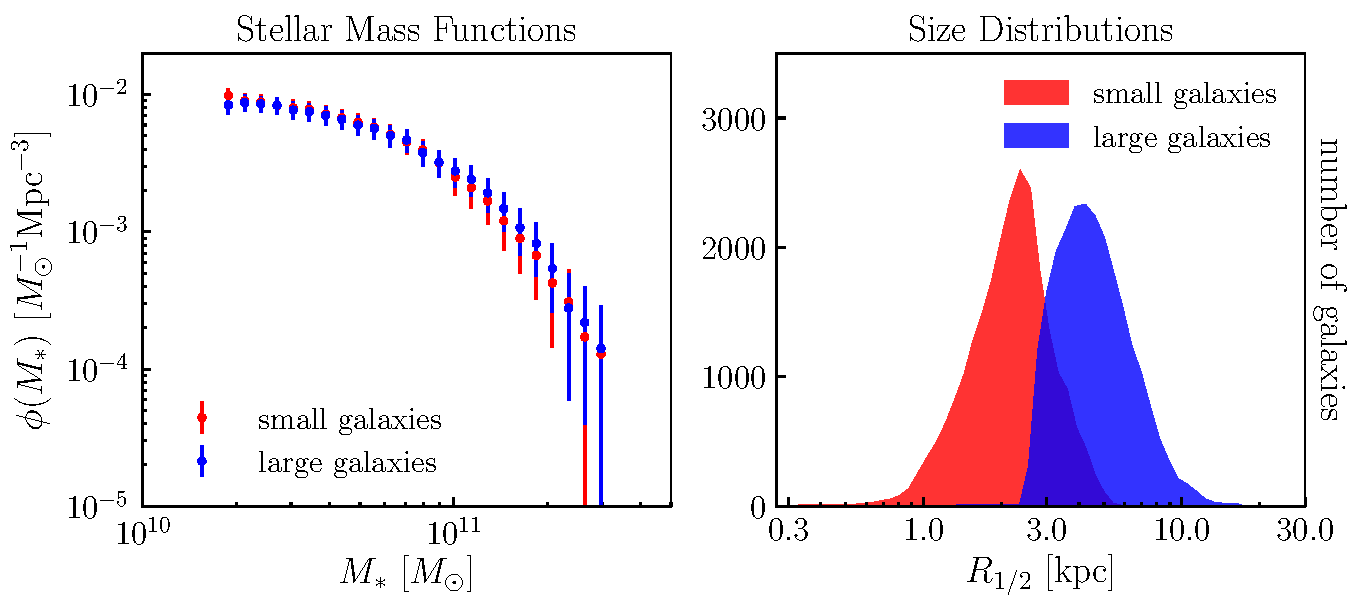
\includegraphics[width=\textwidth]{FIGS/sdss_small_large_sample_definitions.pdf}
\caption{
{\bf Definition of ``small" and ``large" galaxies.} For a volume-limited SDSS galaxy sample defined by $M_{\ast}>10^{10.25}M_{\odot},$ we visually demonstrate how we classify galaxies into ``small" and ``large" subsamples. As described in detail in \S\ref{subsec:sizedef}, we compute the median value $\median{\rhalf}{\mstar}$ at the stellar mass of each galaxy in the sample, and divide the sample into two based on this $\mstar-$dependent cut. The {\em left panel} compares the stellar mass functions $\phi(\mstar)$ of the two samples, confirming that our method for separating ``small" from ``large" galaxies yields subsamples with statistically indistinguishable $\phi(\mstar)$. The {\em right panel} shows histograms of $\rhalf$ for the two subsamples, which partially overlap due to the finite range of $\mstar$ in the volume-limited sample.
}
\label{fig:sizedefinition}
\end{figure*}
%-----------------------------------------------------------------------------------------------------

%-----------------------------------------
\section{Data and Simulations}
\label{sec:data}
%-----------------------------------------

Using galaxies observed in the Data Release 10 of the Sloan Digital Sky Survey \citep[SDSS,][]{ahn_etal14} with the stellar mass measurements taken from the MPA-JHU catalog \citep{kauffmann_etal03,brinchmann_etal04}, we define volume-limited samples of galaxies according to the same $\mstar-$completeness cuts used in \citet{behroozi_etal15} (see Figure 2). We supplement the MPA-JHU catalog with measurements of half-light radius, $\rhalf,$ derived from galaxy profile decompositions provided by \citet{meert_etal15}. The \citet{meert_etal15} catalog is based on Data Release 7 of SDSS \citep{abazajian_etal09}, with improvements to the photometry pipeline and light profile fitting method and, especially, in background subtraction \citep{vikram_etal10,bernardi_etal13,bernardi_etal14,meert_etal13}. In the version of this catalog that we use,\footnote{Our $\mstar$ and $\rhalf$ measurements are derived from different photometry pipelines; this is driven by our desire for consistency with the \citet{behroozi_etal15} completeness cuts used in our clustering measurements. We note that we have repeated our analysis for stellar mass measurements based on \citet{meert_etal15}, finding only minor quantitative, and no qualitative changes to our results.} two-dimensional $r-$band profiles were fit with a two-component de Vaucouleurs + exponential profile to determine the half-light radius of total $r-$band luminosity, $\rhalf.$

As the bedrock of our modeling, we use the publicly available\footnote{\url{http://www.slac.stanford.edu/~behroozi/BPlanck\_Hlists}} catalog of {\tt Rockstar} subhalos identified at $z=0$ in the Bolshoi-Planck simulation \citep{klypin_etal11,behroozi12_rockstar,behroozi12_consistent_trees,riebe_etal13,rodriguez_puebla16_bolplanck}. As described in \S\ref{subsec:sham}, we will use traditional abundance matching to connect stellar mass $\mstar$ with subhalo peak mass $\mpeak.$ To address issues related to subhalo incompleteness \citep{guo_white13,campbell_etal17}, we supplement the Bolshoi-Planck subhalo catalog with subhalos that have been disrupted and no longer appear in the standard catalog as $z=0$ surviving subhalos. We describe our treatment of these ``orphan" subhalos in the Appendix.

For our SDSS galaxy samples, we calculate two-point clustering $\wproj$ using line-of-sight projection of $\pi_{\rm max}=20~\mpc$ using the {\tt correl} program in {\tt UniverseMachine}. For mock galaxies, to compute galaxy clustering we employ the distant observer approximation by treating the simulation $z-$axis as the line-of-sight. We compute $\wproj$ using the {\tt mock\_observables.wp} function in {\tt Halotools} \citep{hearin_etal16}, which is a python implementation of the algorithm in the {\tt Corrfunc} C library \citep{sinha_etal17}. We also use {\tt Halotools} to compute the galaxy-galaxy lensing signal, $\Delta\Sigma,$ using the {\tt mock\_observables.delta\_sigma} function.

All numerical values of $\rhalf$ will be quoted in physical $\kpc,$ and all values of $\mstar$ and $\mhalo$ in $\msun,$ assuming $H_0=67.8~\kms\equiv100h~\kms,$ the best-fit value from \citet{planck15}. To scale stellar masses to ``$h=1$ units" \citep{croton13}, our numerically quoted values for $\mstar$ should be multiplied by a factor of $h^2,$ while our halo masses and distances should be multiplied by a factor of $h.$

\subsection{Classifying large vs. small galaxies}
\label{subsec:sizedef}

Because galaxy clustering has well-known dependence upon $\mstar$ that is not the subject of this work, we wish to remove this influence and focus purely on the relationship between $\rhalf$ and $\wproj(\rproj).$ To do so, we determine the value $\median{\rhalf}{\mstar}$ by computing a sliding median of $\rhalf$ for galaxies sorted by $\mstar,$ calculated using a window of width $N_{\rm gal}=1000.$ Each galaxy is categorized as either ``large" or ``small" according to whether it is above or below the median value appropriate for its stellar mass. We note that this is analogous to the common convention for studying the properties of ``red" vs. ``blue" galaxies, in which the two subsamples are divided by a $\mstar-$ or luminosity-dependent green valley cut \citep[e.g.,][]{vdB_etal08,zehavi_etal11}, only here the $\rhalf$ distribution is uni-modal, not bi-modal.

Using this technique, for any $\mstar-$threshold sample, the stellar mass function of the ``large" and ``small" subsamples are identical. We illustrate this for the particular case of $\mstar>10^{10.25}\msun$ in left panel of Figure~\ref{fig:sizedefinition}, which shows stellar mass functions for the two subsamples. The right panel of Figure~\ref{fig:sizedefinition} compares histograms of the two size distributions of these subsamples, which partially overlap due to the variation in $\median{\rhalf}{\mstar}$ across the $\mstar-$ range of the threshold sample.

In addition to stellar mass, $\wproj(\rproj)$ depends on galaxy color \citep[e.g.,][]{zehavi_etal11}. Thus, we will also consider
dependence of clustering on galaxy size while controlling for color. The results for the subsamples split in stellar mass and color are presented in \S\ref{subsec:colormorph}.

\section{Galaxy-Halo Model}
\label{sec:model}

\subsection{Abundance Matching}
\label{subsec:sham}

We map $\mstar$ onto subhalos using deconvolution abundance matching (SHAM). See section 3.3 of \citet{behroozi_etal10} or the appendix of \citet{kravtsov_etal14} for an account of the mathematics underlying this technique in the presence of scatter. To perform the abundance matching, we use the publicly available code\footnote{\url{https://bitbucket.org/yymao/abundancematching/overview}} developed by Yao-Yuan Mao \citep{lehmann_etal15} that provides a python wrapper around the C kernel developed by Peter Behroozi \citep{behroozi_etal10}. For the subhalo property used in SHAM, we use $\mpeak,$ the largest value of $\mvir$ ever attained by the subhalo throughout the entire history of the main progenitor halo.  Using the stellar mass function provided in \citet{moustakas_etal13}, we model $\mstar$ as a log-normal distribution with $0.2$dex of scatter about the median relation $\median{\mstar}{\mpeak}$ determined by SHAM. As described in the appendix, we include a prescription for supplementing the ordinary {\tt Rockstar} subhalo catalog with disrupted subhalos, so that some of our model galaxies inhabit subhalos that are no longer resolved and do not appear in the standard publicly available catalog.

Figure \ref{fig:baseline_sham_clustering} shows that our implementation of SHAM produces model galaxies whose projected clustering, $\wproj(\rproj)$, is in reasonably good agreement with SDSS galaxies. We note, however, that $\wproj(\rproj\gtrsim1{\rm Mpc})$ is $\sim10-20\%$ too weak at stellar mass $\mstar\gtrsim10^{10.75}\msun.$

%---------------------------------------------------------------------------------------------------
\begin{figure}
\centering
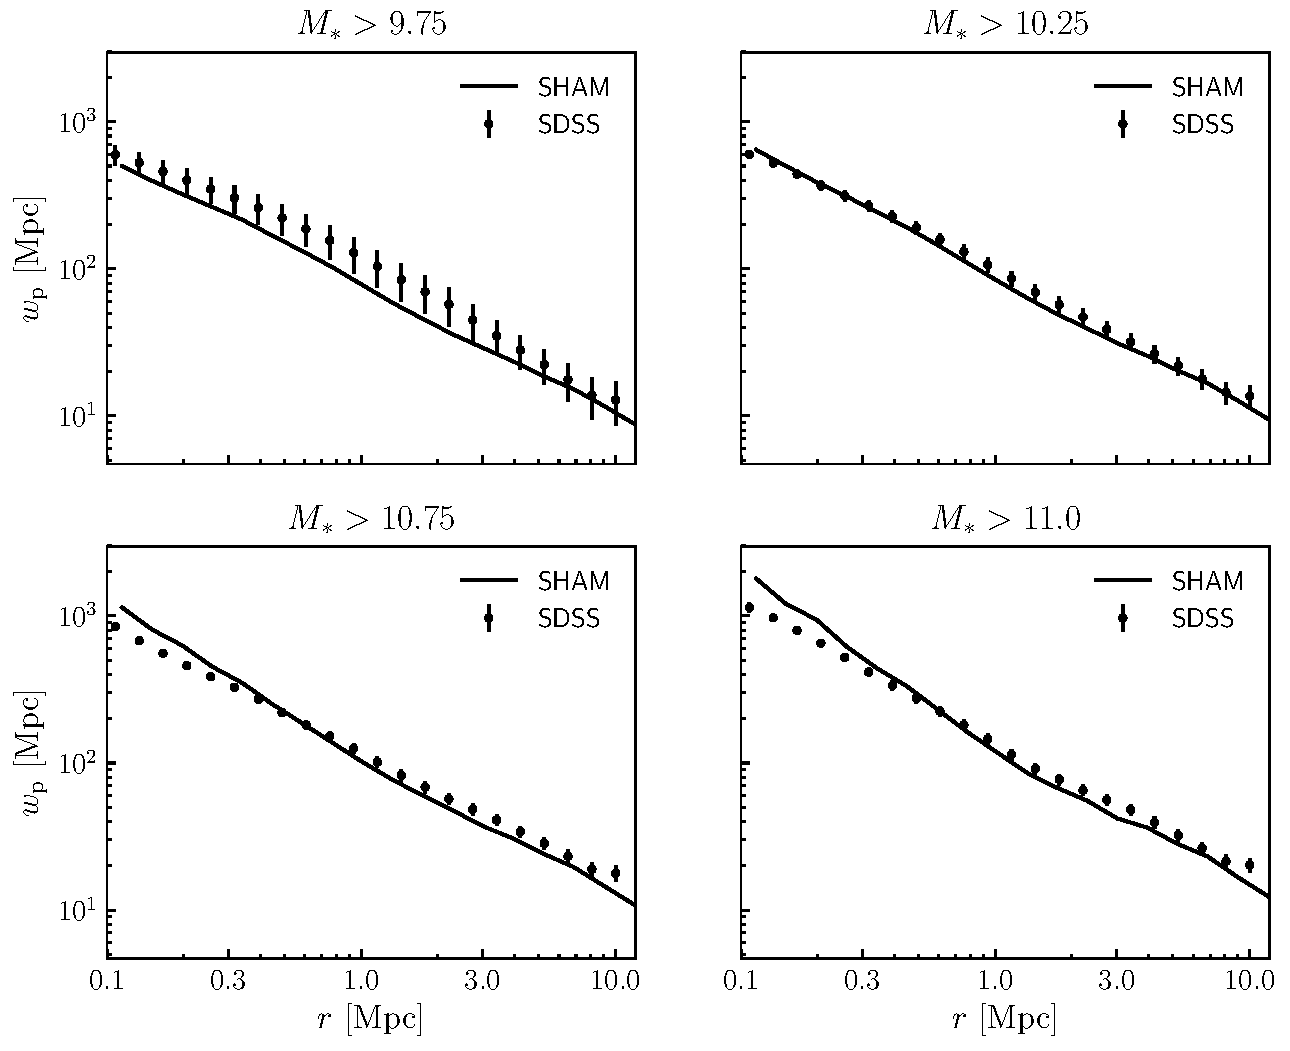
\includegraphics[width=8cm]{FIGS/baseline_sham.pdf}
\caption{
{\bf Abundance matching clustering predictions.}
Using the abundance matching methods described in \S\ref{subsec:sham}, we compare the projected clustering of mock vs. SDSS galaxies. Each panel shows the comparison for a volume-limited sample defined by a different $\mstar-$threshold. Black points with error bars show SDSS measurements; solid black curves show the abundance matching prediction of our fiducial model, which includes the effect of orphan subhalos (see Appendix A). Including orphans mitigates the discrepancy in the clustering predicted by traditional, $\mpeak-$based SHAM based, though mild tension remains on small scales for $\mstar\gtrsim10^{10.75}\msun,$ and on all scales for the $\mstar\gtrsim10^{9.75}\msun.$
}
\label{fig:baseline_sham_clustering}
\end{figure}
%-----------------------------------------------------------------------------------------------------

\subsection{Galaxy size models}
\label{subsec:model}

In \S\ref{sec:results}, we calculate predictions for the $\rhalf-$dependence of galaxy clustering for two classes of empirical models, described in turn below.

\subsubsection{Satellite mass loss model}
\label{subsubsec:strippingmodel}

\textcolor{blue}{AK: I don't think the name of the model is descriptive here, but I could not yet come up with a better one.}
In the first model we explore, we assume that stellar mass $\mstar$ controls $\rhalf,$ so that galaxy sizes are drawn from a log-normal distribution with $0.2$ dex of scatter centered at $\median{\rhalf}{\mstar}.$ To implement this model, for simplicity we tabulate $\median{\rhalf}{\mstar}$ directly from the data, rather than pursue a parametric form \citep[see, e.g.,][]{zhang_yang17}. Note that this model reproduces the observed $\rhalf-\mstar$ relation by construction.


It is natural to consider the possibility that stellar mass is stripped from satellite galaxies after infall. The basis for our implementation of this phenomenon is the fitting function presented in \citet{smith_etal16}, which was calibrated by studying stellar mass loss in a suite of high-resolution hydrodynamical simulations. In this model, $f_{\ast}$ quantifies the remaining fraction of stellar mass as a function of $f_{\rm DM},$ the fraction of dark matter mass that remains after subhalo infall:
\beq
f_{\ast} = 1 - \exp(-14.2f_{\rm DM}).
\eeq
For $f_{\rm DM}$ we use the ratio of present-day subhalo mass divided by the peak mass, $M_{\rm vir}/M_{\rm peak}.$ If we denote the post-stripping stellar mass as $M_{\ast}',$ then we have $M_{\ast}'\equiv f_{\ast}M_{\ast},$ where $M_{\ast}$ is given by the initial application of abundance matching. We then calculate the post-stripping radius by interpolating $\langle\rhalf'\vert\mstar'\rangle$ directly from SDSS data. In this way, we model satellite mass loss and  size truncation in a manner that mimics what is seen in hydrodynamical simulations.


\subsubsection{$\rvir-$based model}
\label{subsubsec:rvirmodel}

%---------------------------------------------------------------------------------------------------
\begin{figure}
\centering
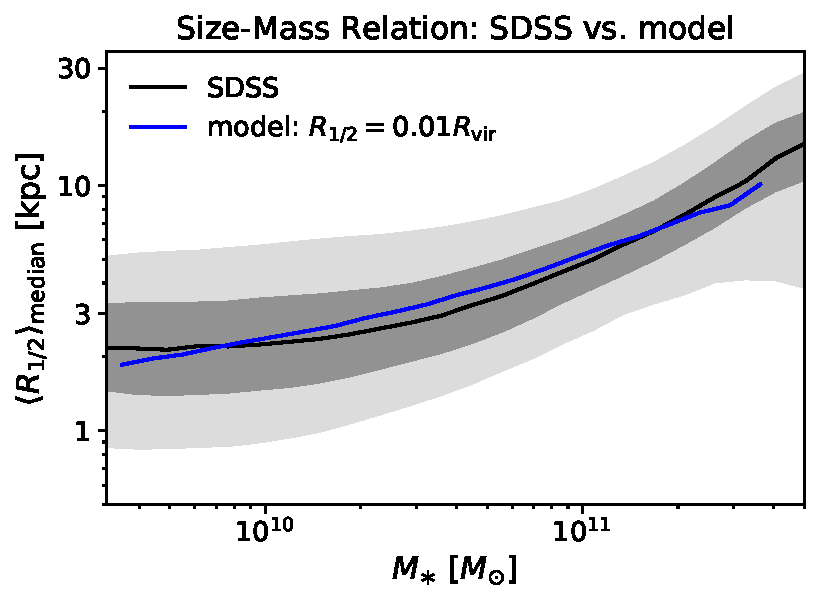
\includegraphics[width=8cm]{FIGS/rvir_only_rhalf_vs_mstar_sham_model.pdf}
\caption{
The black curve shows the median size-mass relation of SDSS galaxies as measured in \citet{meert_etal15}. The two gray bands enveloping the black curve show the $50\%$ and $90\%$ percentile regions. The blue curve shows $\rvir-$based model in which $\median{\rhalf}{\rvir}=0.01\rvir.$ This figure confirms that a linear relationship between $\rvir$ and $\rhalf$ predicts the characteristic curvature in the relation $\median{\rhalf}{\mstar}$ over a wide range in mass.
}
\label{fig:scatter_plot}
\end{figure}
%-----------------------------------------------------------------------------------------------------

%---------------------------------------------------------------------------------------------------
\begin{figure*}
\centering
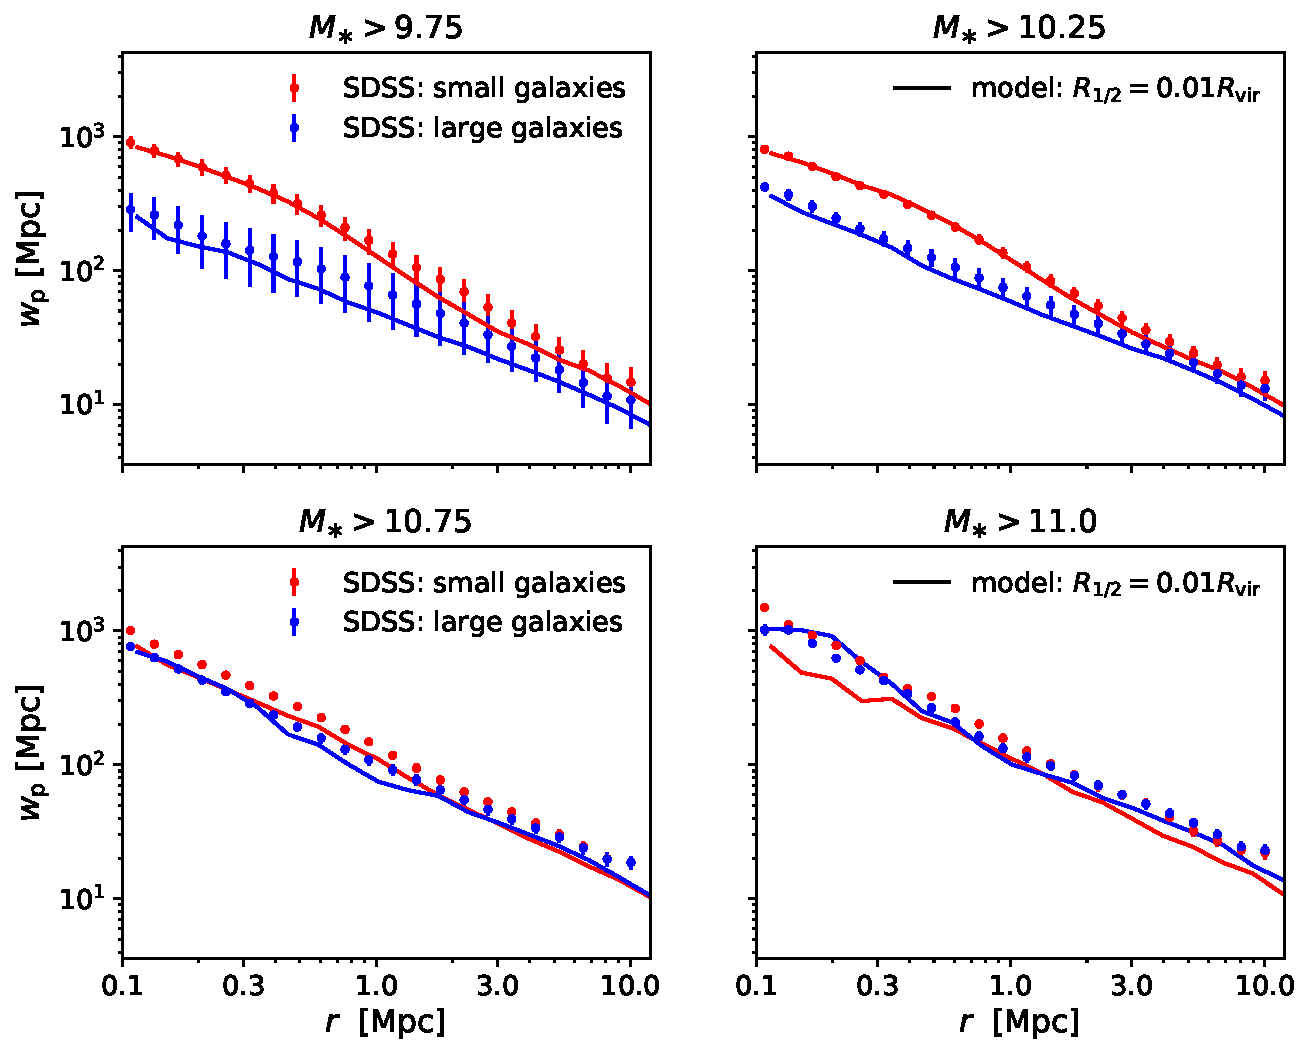
\includegraphics[width=12cm]{FIGS/rvir_only_wp_large_small_absolute.pdf}
\caption{
{\bf $\rhalf-$dependence of galaxy clustering.}
Red and blue points with error bars show our SDSS measurements of the clustering of small and large galaxies, respectively. For each volume-limited sample of $\mstar-$complete galaxies, the small and large subsamples have identical stellar mass functions, as shown in Figure \ref{fig:sizedefinition}. Small galaxies cluster much more strongly relative to large galaxies of the same stellar mass. Solid curves show the clustering predictions of the $\rvir-$based model described in \S\ref{subsubsec:rvirmodel}. The $\rvir-$based model inherits the shortcoming of ordinary abundance matching shown in Figure \ref{fig:baseline_sham_clustering}, although the model faithfully captures the {\em relative} clustering of small vs. large galaxies, as shown in Figure \ref{fig:clustering_ratio_upshot}.
}
\label{fig:rvir_only_clustering_absolute}
\end{figure*}
%-----------------------------------------------------------------------------------------------------

%---------------------------------------------------------------------------------------------------
\begin{figure*}
\centering
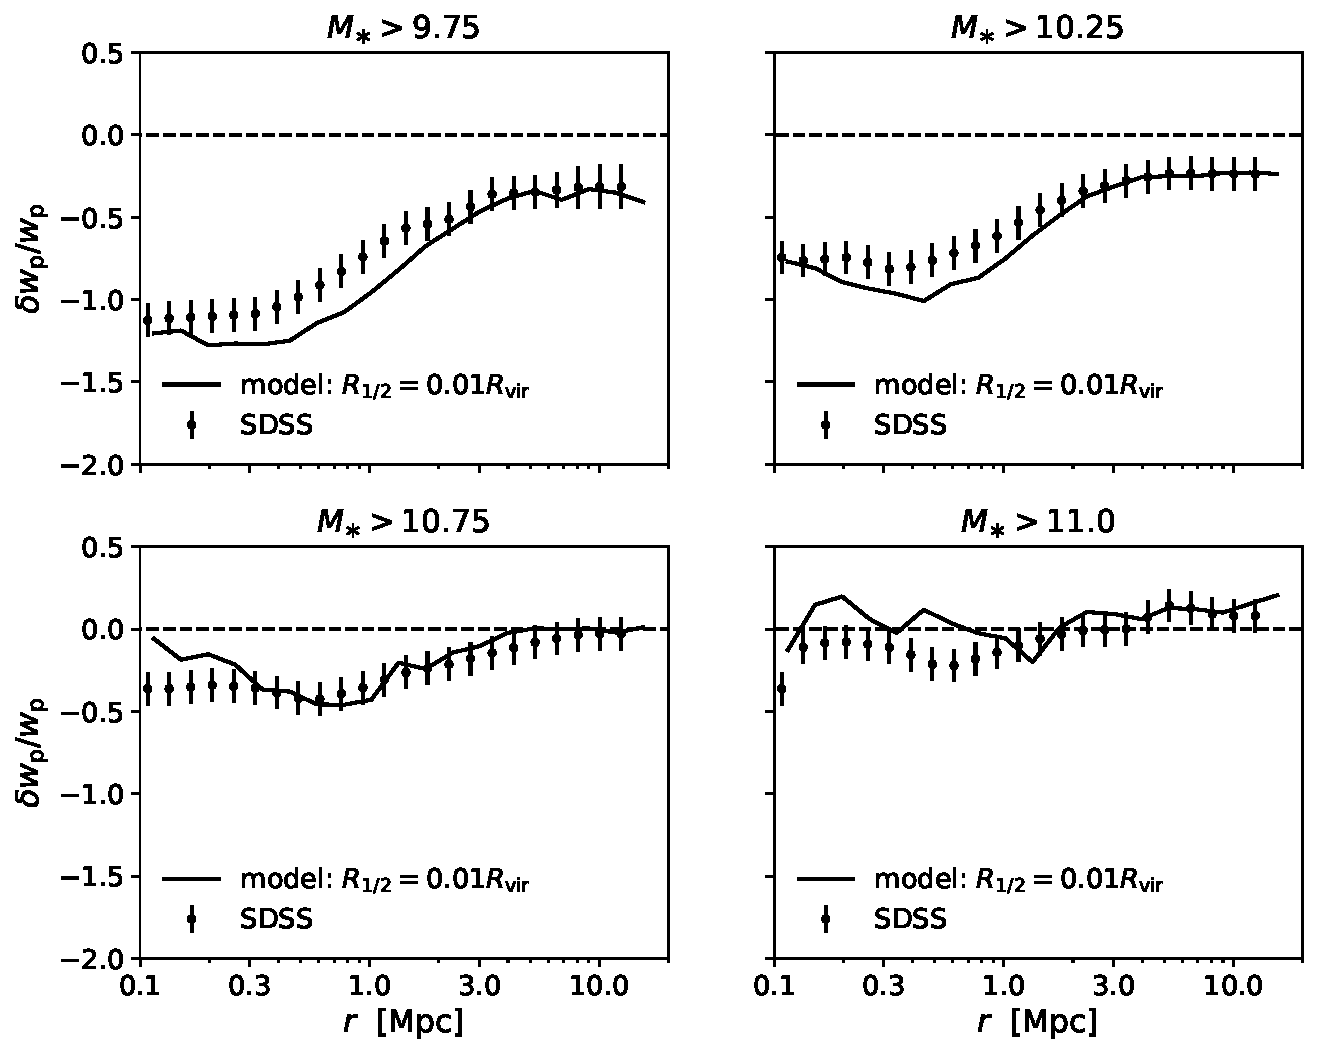
\includegraphics[width=12cm]{FIGS/rvir_only_wp_ratios.pdf}
\caption{
{\bf $\rhalf-$dependence of galaxy clustering: clustering ratios.}
Closely related to Figure \ref{fig:rvir_only_clustering_absolute}, the y-axes show {\em clustering strength ratios,} defined as $(w_{\rm p}^{\rm large} - w_{\rm p}^{\rm small})/w_{\rm p}^{\rm all}.$ Thus a y-axis value of $-0.5$ corresponds to small galaxies being $50\%$ more strongly clustered than large galaxies of the same stellar mass. Solid curves show the clustering ratio predictions of the $\rvir-$based model described in \S\ref{subsubsec:rvirmodel}. Normalizing the measurements and predictions by $w_{\rm p}^{\rm all}$ scales away the shortcoming of ordinary abundance matching (see Figure \ref{fig:baseline_sham_clustering}), highlighting the successful prediction of the $\rvir-$based model for the $\rhalf-$dependence of galaxy clustering.
}
\label{fig:clustering_ratio_upshot}
\end{figure*}
%-----------------------------------------------------------------------------------------------------


As noted in \S\ref{sec:intro}, \citet{kravtsov13} showed that galaxy sizes are on average proportional to the virial radius of their host halo. Motivated by these results, we  explore a model in which $\rhalf$ scales linearly with the halo virial radius:\footnote{We note that the normalization factor in \citet{kravtsov13} is 0.015, where as our normalization is 0.01. The difference derives from two factors: {\em i.} the choice of halo radius definition: \citet{bryan_norman98} in the present work, compared to the $200c$ definition used in \citet{kravtsov13}; {\em ii.} the latter study used deprojected (larger) sizes for spheroidal galaxies, whereas we make no such correction here.}
\beq
\label{eq:fiducial_model}
\rhalf = 0.01\rvir.
\eeq
For the virial radius of halos and subhalos, we use $\rmpeak:$ the value of $\rvir$ in physical units of $\kpc$ measured at the time when halo mass reached its maximum.  The relationship between $\rmpeak$ and $\mpeak$ is given by
\beq
\mpeak\equiv\frac{4\pi}{3}\rmpeak^{3}\Delta_{\rm vir}(\zpeak)\rho_{\rm m}(\zpeak),
\eeq
where for $\Delta_{\rm vir}(\zpeak)$ we use the fitting function to the ``virial" definition used in \citet{bryan_norman98}. For the model we refer to as the ``$\rvir-$based model", we add uncorrelated log-normal scatter of $\sigmarhalf=0.2$ dex to generate a Monto Carlo realization of the model population.

%-----------------------
\section{Results}
\label{sec:results}
%-----------------------

%--------------------------------------------------------
\subsection{Size-Mass Scaling Relation}
\label{subsec:one_point_function}
%-------------------------------------------------------

In Figure \ref{fig:scatter_plot} we show the scaling of galaxy size $\rhalf$ with $\mstar.$ The black curve enveloped by the gray bands shows the scaling relation for SDSS galaxies, while the blue curve shows the median relation  $\median{\rhalf}{\mstar}$ predicted using the $\rvir-$based model described in \S\ref{subsubsec:rvirmodel}. This figure shows that models in which $\rhalf\propto\rvir$ can naturally match the observed $\rhalf-\mstar$ relation, confirming the results of \citet{kravtsov13} in a forward modeling context.

%---------------------------------------------------------------------------
\subsection{Size-Dependent Clustering Measurements}
\label{subsec:clustering_results}
%---------------------------------------------------------------------------

In Figure~\ref{fig:rvir_only_clustering_absolute}, we present new measurements of the $\rhalf-$dependence of projected galaxy clustering, $\wproj(\rproj).$ We measure $\wproj(\rproj)$ separately for large and small subsamples for four different $\mstar$ thresholds, $\mstar>10^{9.75}\msun,$ $\mstar>10^{10.25}\msun,$ $\mstar>10^{10.75}\msun,$ and $\mstar>10^{11}\msun.$ For each threshold, we split the galaxies into ``large" and ``small" subsamples, as described in \S\ref{subsec:sizedef}. As shown in Figure \ref{fig:sizedefinition}, our size-based samples  have similar stellar mass functions. Red points with jackknife-estimated error bars show SDSS measurements of $\wproj(\rproj)$ for samples of small galaxies, while blue points show the measured correlation functions for samples of large galaxies. Solid curves show $\wproj$ as predicted for these subsamples by the $\rvir-$based model of galaxy sizes described in \S\ref{subsubsec:rvirmodel}.

The salient feature of these clustering measurements is that small galaxies cluster more strongly than large galaxies of the same stellar mass in all but the largest $\mstar$ samples. Remarkably, both the trend and the quantitative difference in the shape of the correlation functions of small and large galaxy samples are reproduced by the $\rvir-$based model. This may be surprising, since $\rhalf\propto\rvir,$ halo mass $\rvir\propto\mhalo^{1/3},$ and clustering strength of halos increases with $\mvir.$ Based on this simple argument, one would expect that large galaxies would be the more strongly clustered. We provide a resolution to this conundrum in \S\ref{subsec:censat_sizes}. However,  before doing so, we first examine the clustering test of the $\rvir-$based model in more detail.

As shown in Figure \ref{fig:baseline_sham_clustering}, the abundance matching prediction for $\wproj(\rproj)$ exhibits tension with SDSS observations at the $10-20\%$ level, particularly for $\mstar\gtrsim10^{10.75}\msun.$ This tension is inherited by our $\rvir-$based model for size, which is the subject of this work, and so we wish to compare our size models to data in such a way that minimizes the role played by the underlying stellar-to-halo-mass relation. We accomplish this using {\em the $\rhalf$ clustering ratios,} described below.

For each volume-limited $\mstar-$threshold sample, we additionally measure $\wproj(\rproj)$ {\em without} splitting on size, giving us measurements $\wpall, \wplarge,$ and $\wpsmall$ for each threshold sample. This allows us to compute the ratio $(\wplarge-\wpsmall)/\wpall,$ which we refer to as {\em the $\rhalf$ clustering ratio}. These ratios, denoted as $\delta\wproj/\wproj,$ are the measurements appearing on the y-axis in each panel of Figure \ref{fig:clustering_ratio_upshot}. As a specific example, a clustering ratio of $-0.5$ corresponds to small galaxies being $50\%$ more strongly clustered than large galaxies of the same stellar mass.

The points and curves in Figure \ref{fig:clustering_ratio_upshot} are all negative: small galaxies cluster more strongly relative to large. This presentation of the measurement makes it clear that the underlying signal of $\rhalf-$dependent clustering is strongest for samples with smaller stellar mass; as $\mstar$ increases, the signal weakens and nearly vanishes for $\mstar\gtrsim10^{11}\msun.$ Strikingly, the $\rvir-$based model reproduces this $\mstar-$dependent behavior, as well as the scale-dependence of the observed clustering signal at each $\mstar.$ As described in \S\ref{subsec:censat_sizes} below, we attribute the success of this prediction to the systematic difference of sizes of central and satellite galaxies.

%--------------------------------------------------------------------------
\subsection{Testing the Impact of Satellite Mass Loss}
\label{subsec:mstar_stripping}
%--------------------------------------------------------------------------------------
\begin{figure*}
\centering
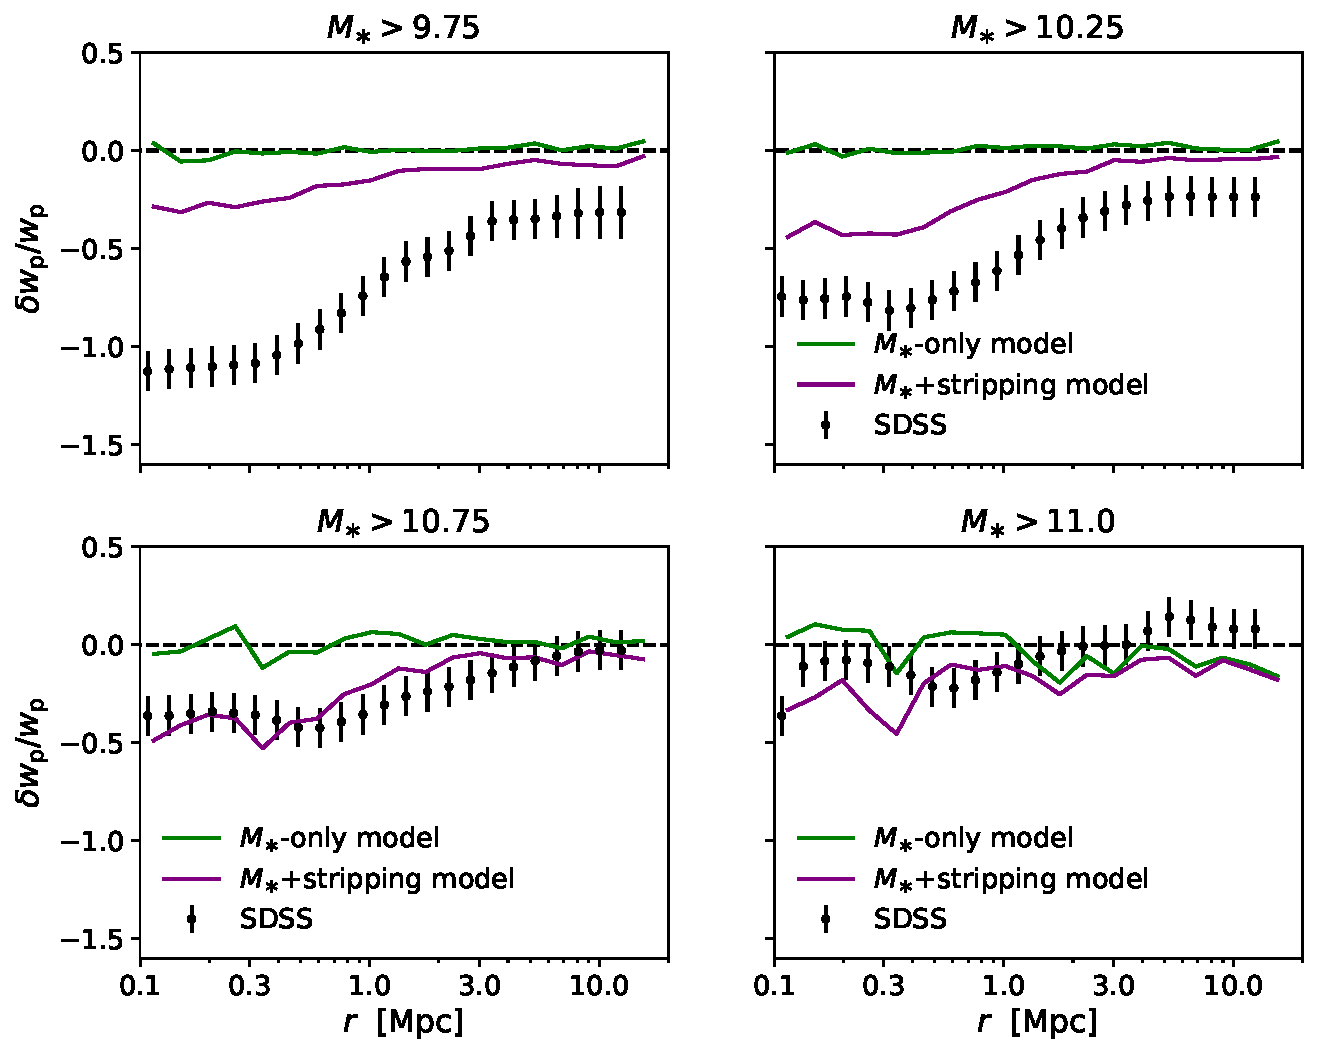
\includegraphics[width=12cm]{FIGS/alt_model_wp_ratios.pdf}
\caption{
{\bf The subdominant role of tidal stripping.}
In all panels, the axes and points with error bars are the same as in Figure \ref{fig:clustering_ratio_upshot}. The solid green curves shows the prediction of a model where $\rhalf$ is statistically set by $\mstar,$ in the complete absence of satellite mass loss. Such a model would predict zero $\rhalf-$dependence to galaxy clustering, in gross tension with observations. The solid purple curves show results for a model in which satellites lose mass after infall in a manner similar to what is seen in high-resolution hydrodynamical simulations, as described in \S\ref{subsubsec:strippingmodel}. This produces satellites that are smaller than centrals, but the effect is too mild to correctly capture the observed clustering. Evidently, satellite-specific mass stripping plays a sub-dominant role in setting the relative size of centrals and satellites.
}
\label{fig:mstarmodelclustering}
\end{figure*}
%-----------------------------------------------------------------------------------------------------

Figure~\ref{fig:mstarmodelclustering} shows a similar comparison of the observed clustering ratios to the model
in which size is controlled by $\mstar$ with sizes of satellites affected by stellar mass loss due to tides (\S\ref{subsubsec:strippingmodel}). Green solid lines show predictions of the model that does not account for stellar
mass loss of satellites due to tides. In this model $\rhalf$ follows a purely random log-normal distribution centered at $\median{\rhalf}{\mstar}$ with the median relation matched to the observed relation by construction.  This model thus predicts no dependence of galaxy clustering upon $\rhalf$ at fixed $\mstar,$ simply because the scatter of $\rhalf$ about $\median{\rhalf}{\mstar}$ is uncorrelated with any other variable. The figure shows that this model clearly is at odds with significant dependence of clustering on size exhibited by SDSS galaxies.

Inclusion of satellite mass loss in the model introduces correlations in the scatter: after mass loss, satellites have smaller sizes than centrals of the same $\mstar$ due to post-infall stripping.
The purple curves in Figure \ref{fig:mstarmodelclustering} show that satellite mass loss impacts $\rhalf-$dependent clustering in the expected manner. The ``small" galaxy population has a higher satellite fraction due to satellites being smaller than centrals of the same $\mstar,$ and so in this model small galaxies cluster more strongly relative to large. However, the magnitude of the effect is not sufficiently strong  to produce clustering predictions that are consistent with observations. Evidently it is difficult to strip enough mass from satellites so that the $\rhalf-$dependent clustering predictions are in agreement with observations.  We reach the same conclusion when we tested an even more extreme $\mstar-$stripping model, in which stellar mass loss is linearly proportional to halo mass loss \citep[][Model 1]{watson_etal12}.
As we argue in \S\ref{sec:interpretation}, this supports the conclusion that the relative difference between central and satellite size is largely in place at the time of satellite infall.

%----------------------------------------------------
\subsection{The Role of Galaxy Color}
\label{subsec:colormorph}
%----------------------------------------------------

We now examine how galaxy clustering depends on size when we control both for stellar mass and color dependence of galaxy clustering. Using the $\mstar>10^{10.25}\msun$ sample used above, we first divide the sample into ``red" and ``blue" subsamples using $g-r=0.65$ as a boundary, which approximately corresponds to the trough of the green valley for this stellar mass. For each color-selected subsample, we separately measure $\median{\rhalf}{\mstar; {\rm red}}$ and $\median{\rhalf}{\mstar; {\rm blue}},$ and use these median size values to split each subsample into two.

Figure \ref{fig:colorclustering} shows the clustering of large vs. small galaxies, separately for red and blue samples. For each color-selected sample, large galaxies are slightly more strongly clustered relative to small galaxies. Comparing Figure \ref{fig:colorclustering} to the the upper right panel of Figure \ref{fig:rvir_only_clustering_absolute} shows the size dependence for color-selected samples is dramatically weaker.   For $\mstar-$complete samples, small galaxies cluster much stronger than large galaxies; for color-selected samples, the reverse is true, but the difference is much smaller and is confined to a limited range of scales.  Although the two results may seem surprising, even contradictory, they can, in fact be
explained within a unified simple model, as will be discussed in \S\ref{sec:interpretation}.

%---------------------------------------------------------------------------------------------------
\begin{figure*}
\centering
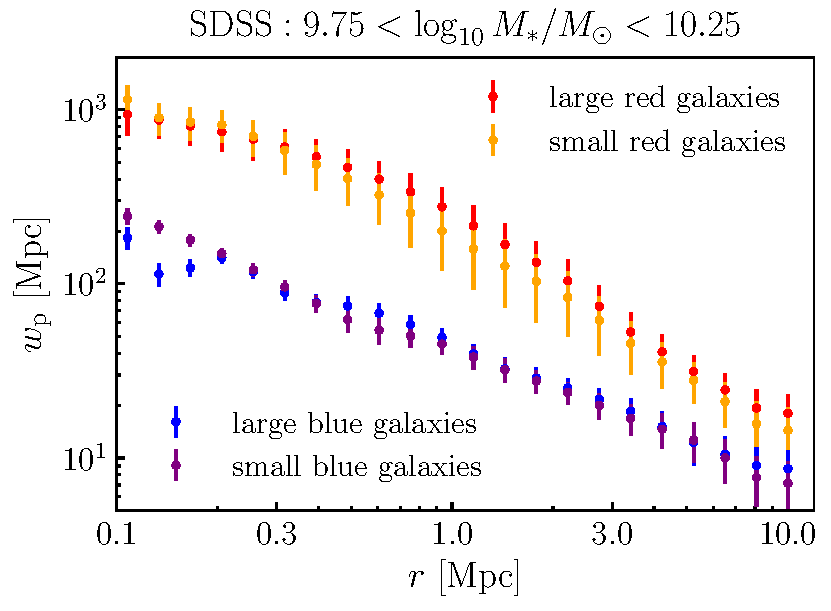
\includegraphics[width=8cm]{FIGS/color_selected_size_dependent_clustering.pdf}
\caption{
{\bf Distinct $\rhalf-$dependence of clustering for color-selected galaxy samples.}
Projected clustering of SDSS galaxies in the bin of stellar mass: $10^{9.75}<\mstar/\msun<10^{10.25}.$ For both ``blue" and ``red" samples, we first divide SDSS galaxies falling in the $\mstar$ bin based on a color cut at $g-r=0.65.$ We then subsequently compute $\median{\rhalf}{\mstar; {\rm red}}$ and $\median{\rhalf}{\mstar; {\rm blue}}$. In analogy to the left panel of Figure \ref{fig:sizedefinition}, this sample definition results in identical stellar mass function for large and small subsamples, separately for both red and blue parent samples. We then measure $\wproj$ for each of the four subsamples, plotting the results with color-coding as specified in the legend. At this stellar mass, pre-selecting galaxy samples by color results in a dramatic weakening of the $\rhalf-$dependence of $\wproj$ relative to $\mstar-$complete samples, as well as a sign-reversal of the signal.
}
\label{fig:colorclustering}
\end{figure*}
%---------------------------------------------------------------------------------------------------


%---------------------------------------------------------------------------------------------------
\begin{figure}
\centering
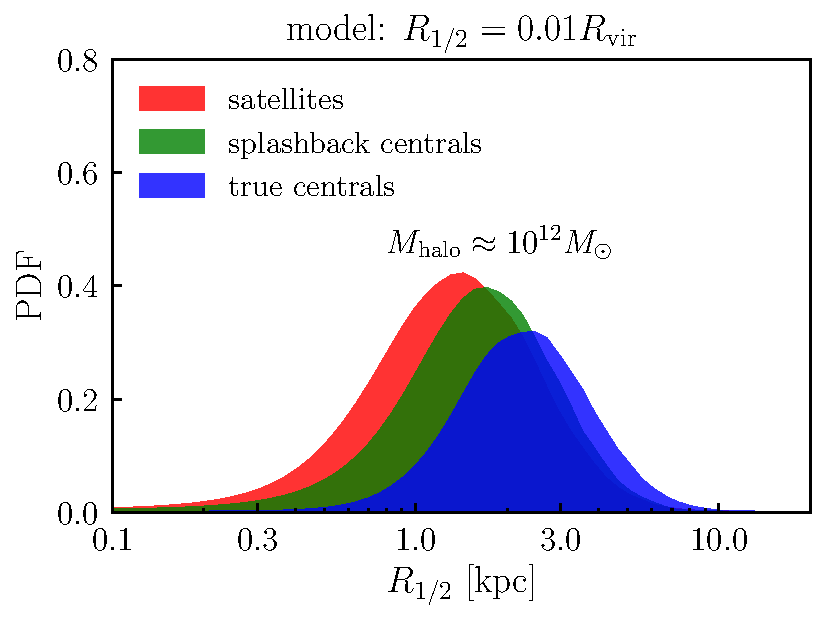
\includegraphics[width=8cm]{FIGS/rvir_only_cen_sat_sizes.pdf}
\caption{
{\bf Relative sizes of centrals and satellites.}
In a narrow bin of halo mass $\mhalo\equiv\mpeak\approx10^{12}\msun,$ we show the distribution of model galaxy sizes for different subpopulations galaxies, as predicted by the $\rvir-$based model. The red histogram shows the sizes of satellites; the blue histogram shows host halos that have never passed inside the virial radius of a larger halo (``true centrals"); the green histogram host halos that were subhalos inside a larger at some point in their past history (``splashback centrals"). In the $\rvir-$based model, galaxy size is set by the {\em physical} size of the virial radius at the time the halo attains its peak mass, naturally resulting in smaller sizes for satellites and splashback centrals relative to true centrals of the same $\mhalo.$
}
\label{fig:censatsizehist}
\end{figure}
%-----------------------------------------------------------------------------------------------------


%-----------------------------------------------------------------------------------------
\section{A Unified Interpretation of $\rhalf-$Dependent Clustering}
\label{sec:interpretation}
%-----------------------------------------------------------------------------------------

In the previous section, comparing model predictions to the observed size dependence of galaxy clustering produced two intriguing results. First, the model that assumes $\rhalf\propto\rvir$ predicts a dependence of both the amplitude and shape of  galaxy correlation functions on size remarkably well, especially considering that the model nominally has only one free parameter: the normalization of the linear $\rhalf-\rvir$ relation. At the same time, small galaxies cluster more strongly relative to large, which seems at odds with naive expectations that, within such a model, larger sizes correspond to larger halo masses, $\rvir\propto\mvir^{1/3}$, and so larger sizes should be clustered more strongly. Second, the strong dependence of galaxy clustering on size weakens to almost no dependence for samples of red and blue galaxies selected by color within a given stellar mass range.
Below we propose a simple and unified explanation of all these results within the $\rvir$-based size model in \S\ref{subsec:censat_sizes}, and discuss the broader implications of our interpretation in \S\ref{subsec:broader_implications}.

%----------------------------------------------------------------------------
\subsection{The Relative Size of Centrals vs. Satellites}
\label{subsec:censat_sizes}
%----------------------------------------------------------------------------

Recall that in the $\rvir$-based size model, galaxy size is proportional to the virial radius of host halo at the redshift  when the halo halo attained its maximum mass. Thus, we can expect that in this model satellite galaxies will have sizes smaller than sizes of central galaxies hosted by halos of similar stellar mass.  Indeed, Figure \ref{fig:censatsizehist} shows the $\rhalf$ distributions of central, satellite, and ``splashback'' central galaxies hosted by halos of the same mass $\mhalo\equiv\mpeak\approx10^{12}\msun.$ A ``splashback central"  is defined as a present-day central galaxy that used to be a satellite, i.e., its main progenitor halo passed inside the virial radius of a larger halo at some point in its past history. On the other hand, we define a ``true central" as a galaxy that has never been a satellite. The figure shows that there is a clear trend of sizes decreasing from the central to splashback and to satellite galaxies.

In the $\rvir-$based model, satellites and splashback galaxies are smaller than centrals of the same halo mass due to the physical size of their halo being smaller at earlier times $\zpeak.$ There are two distinct reasons why this feature results in small galaxies being more strongly clustered relative to larger galaxies of the same mass. First and foremost, satellite galaxies statistically occupy higher mass host halos that are more strongly clustered. So in models where satellites are smaller than centrals of the same mass, smaller galaxies will have a higher satellite fraction, boosting the clustering of small relative to large galaxies of the same stellar mass. Second, at fixed mass, halos of $L_\ast$ galaxies that form earlier are more strongly clustered, a phenomenon commonly known as {\em halo assembly bias} \citep{gao_white05,wechsler_etal06}. Splashback halos are typically earlier-forming than true centrals \citep{wang_etal09}, and so models where splashback halos host smaller-than-average galaxies will naturally predict smaller galaxies being the more strongly clustered \citep[see][for an example of the splashback-dependence of halo clustering]{sunayama_etal16}.

We can also understand how the observed $\rhalf-$dependent clustering scales with $\mstar$ (shown by comparing different panels in Figure \ref{fig:clustering_ratio_upshot}) in terms of the differences of sizes of central and satellites galaxies. The satellite fraction $F_{\rm sat}(\mstar)$ decreases as $\mstar$ increases \citep[e.g.,][]{guo_etal11,reddick_etal13}. As $F_{\rm sat}$ decreases, there are fewer satellites available to preferentially weight the subsample of smaller galaxies. Thus,  high $\mstar$ samples consist mostly of central galaxies, and the split by size no longer corresponds to the split into satellite- and central-dominated samples. The size dependence of clustering correspondingly weakens and nearly disappears for samples with largest $\mstar$.

Likewise, the significantly weaker dependence of clustering on size for color-selected samples (Figure \ref{fig:colorclustering}), and its reversed sign, can be naturally explained within the same framework.  For example, it is well known that satellites are redder than centrals of the same stellar mass \citep[e.g.,][]{vdB_etal08}; accordingly, red galaxies cluster much more strongly than  blue galaxies \citep[e.g.,][]{zehavi_etal11}. Samples of red (blue) galaxies with stellar masses of $\mstar\sim 10^{10}\ M_\odot$ are dominated by satellite (central) galaxies, and splitting by size within such samples no longer corresponds to the split into satellite- and central-dominated samples. In this case, the $\rvir$-based size model predicts that splitting by size {\em does} correspond to splitting by halo mass $\rhalf\propto\rvir\propto\mhalo^{1/3},$ and therefore that large galaxies should be somewhat more clustered than the small ones. That is, the $\rvir-$based model predicts that $\rhalf-$dependent clustering should be reversed for color-selected samples, and that the magnitude of the dependence should be significantly weaker due to weak dependence of virial radius on halo mass, and weak dependence of clustering on halo mass in this regime.

While we consider such an explanation plausible, and even likely, a conclusive confirmation requires proper forward modeling of size and color jointly. Such an effort is strongly motivated by our results, but is beyond the scope of the present work.

%-------------------------------------------------
\subsection{Broader Implications}
\label{subsec:broader_implications}
%-------------------------------------------------

The success of the $\rvir$-based model in explaining the size dependence of galaxy clustering implies that the sizes of {\it all} galaxies,  red, blue, spheroid, disks, satellites and central, are, on average, proportional to the $\rmpeak,$ the physical size of the virial radius at the time at which $\mhalo$ stops growing. Although correlation is not necessarily causation, such a universal and simple dependence poses a useful challenge to fine-grained galaxy formation models, as it indicates tight connection between the growth of galaxies and their host halos.

The $\rvir$-based size model assumes as an ansatz that galaxy size remains approximately constant after a halo stops growing; as shown in Figure \ref{fig:clustering_ratio_upshot}, this assumption is consistent with the observed size-dependence of galaxy clustering in SDSS.  The halos of typical satellites reach $\mpeak$ far outside the virial radius of their ultimate host halo \citep{behroozi_etal14}, and so in the $\rvir-$based model the size difference between satellites and centrals is largely in place prior to the time of satellite infall. Halos of central and satellite galaxies of the same $\mstar$ differ in the epoch $\zpeak$ at which their halo stopped growing, and this difference gives a natural explanation for their different median sizes.

This difference also explains the relative trends of $\rhalf-\mstar$ relations for red and blue, or disk and spheroid galaxies.
Both types of galaxies exhibit weak dependence of $\rhalf$ on $\mstar$ at $\mstar\lesssim 5\times 10^{10}\ M_\odot$ and
at these masses $\rhalf$ of disks is a factor of two larger than those of spheroids. At larger masses, the sizes of galaxies of both types show stronger dependence on $\mstar,$ and the difference in median size of disk and spheroid galaxies decreases \citep[e.g.,][]{bernardi_etal14}.

In the $\rvir$-based size model, the weak dependence of $\rhalf$ on $\mstar$ for low-mass galaxies is due to the steep $\mstar-\mvir$ relation. For example, if $\mstar\propto\mvir^\alpha\propto\rvir^{3\alpha}$, then $\rhalf\propto \rvir\propto \mstar^{1/(3\alpha)}$. Given that $\alpha\sim 1-3$ is inferred for the $\mstar-\mvir$ relation at low masses \citep{kravtsov10,moster_etal13,behroozi13_smhm,kravtsov_etal14}, the $\rhalf-\mstar$ relation in this regime is expected to be shallow.
For galaxies of $\mstar\gtrsim 5\times 10^{10}\ M_\odot$, $\alpha\approx 0.3$ \citep[e.g.,][]{kravtsov_etal14}, and thus
the slope of the $\rhalf-\mstar$ relation is approximately linear. These trends of $\rhalf$ with $\mstar$ have a direct relation to the trends of surface brightness $\mu_\star=\mstar/(\pi\rhalf^2)$ with stellar mass \citep[see, for example, the $\mu_\star-$dependent clustering measurements in][which are qualitatively similar to the measurements reported here]{li_etal06}.

The difference in median sizes of disk and spheroidal galaxies at $\mstar\lesssim 10^{11}\ M_\odot$ can be explained by the sizes of satellite galaxies being systematically smaller than the sizes of central galaxies of the same $\mstar,$ coupled with the fact that the satellite fraction is much larger among spheroidal galaxies compared to disk galaxies. For example, the analysis in \citet{rodriguez_puebla_etal15} shows that in this regime, the satellite fraction of blue galaxies is only $\sim10-20\%$, while
the satellite fraction of red galaxies is $\gtrsim 30-50\%,$ increasing with decreasing stellar mass.
As $\mstar$ increases, the satellite fractions of both blue and red galaxies drop, and at $\mstar\gtrsim 10^{11}\ M_\odot,$ the vast majority of blue and red galaxies are centrals. If these galaxies occupy similar halo masses at the same $\mstar$, then the $\rvir$-based size model predicts that the difference in sizes of red and blue galaxies should disappear at these masses, as is indeed observed. A testable prediction of this picture is that when 3D (de-projected) sizes of only central red and blue galaxies of the same $\mstar$ are compared, the sizes should be much closer than the sizes of the overall red and blue populations.



%The broad features of the $\wproj(\rproj)$ measurements shown in Figure \ref{fig:colorclustering} give insight into the characteristics that should be exhibited by any model for the relationship between $B/T$ and $\rhalf.$ First, the bottom right panel of Figure \ref{fig:colorclustering} indicates that the size of the bulge has only a tenuous connection to the properties of its parent dark matter halo.\footnote{Strictly speaking, the size of the bulge could in principle be closely connected to any number of dark matter halo properties, so long as those halo properties do not significantly impact two-point clustering.} Second, for disk-dominated galaxies, the observed $\rhalf-$dependent clustering suggests that at fixed $\mstar,$ the size of the disk is strongly correlated with whether or not the galaxy is a satellite. These findings imply that bulge prominence is intimately connected with the quenching of star-formation, but that there is wide variation in star-formation histories amongst disk-dominated galaxies, in agreement with numerous previous findings \citep[see, e.g.,][]{woo_etal15,font_etal17}.

% A possibly overkill caveat paragraph:
%While these clustering measurements give supporting evidence that satellite mass stripping plays a sub-dominant role in shaping galaxy size, we point out that our treatment of satellite mass loss is only approximate: we have modified the size of satellites without self-consistently modifying total stellar mass. In the present work, we have opted not to develop and fine-tune a complex, semi-analytic model; instead, we have made a simple ``first-order" estimate for the level at which satellite-specific stripping impacts the two-point function. Our findings support the idea that the small sizes of satellites arise primarily from the satellite's distinctive evolution within a high density region and a steep tidal field {\em prior} to becoming a present-day satellite.

%---------------------------------------------------------------------------------------------------
\begin{figure}
\centering
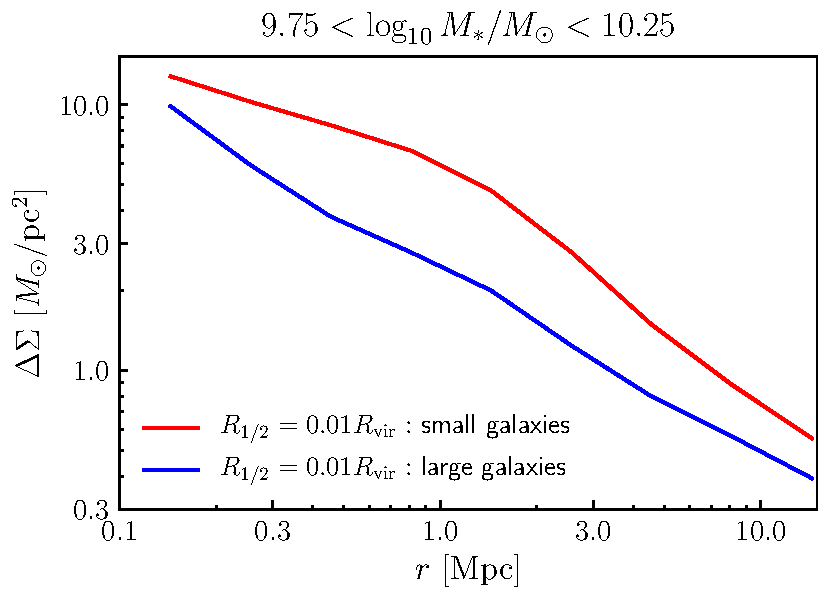
\includegraphics[width=8cm]{FIGS/rvir_only_lensing_prediction.pdf}
\caption{
{\bf Prediction for $\rhalf-$dependence of galaxy lensing.}
Using the $\rvir-$based model described in \S\ref{subsubsec:rvirmodel}, we make predictions for as-yet-unseen measurements of the $\rhalf-$dependence of galaxy lensing of $\mstar-$complete samples, where ``small" and ``large" subsamples are defined as in \S\ref{subsec:sizedef}. As a generic consequence of satellites being smaller than centrals of the same mass, we predict that future lensing measurements of $\mstar-$complete samples will show $\Delta\Sigma$ of small galaxies to be significantly stronger relative to large galaxies of the same stellar mass. To date, the $\rhalf-$dependence of $\Delta\Sigma$ has only been measured for color-selected samples \citep{charlton_etal17}, in which the trend is reversed and weakened: for both blue and red samples, $\Delta\Sigma$ of large galaxies is (slightly) stronger relative to small galaxies.
}
\label{fig:lensingprediction}
\end{figure}
%-----------------------------------------------------------------------------------------------------

\section{Relation to Previous Work}
\label{sec:previous_work}

Numerous previous analyses have employed the \citet{yang_etal05b} group catalog to ``directly" study the relationship between galaxy mass, size, and environment. For example, by treating observed groups as genuine dark matter halos, several analyses have found that the $\mstar-\rhalf$ relation of early-type galaxies exhibits weak, if any, environmental dependence \citep{weinmann_etal08,huertas_company_etal13b,shankar_etal14}. 

As shown in \citet{campbell_etal15}, group-finding methods are subject to significant systematics, particularly when analyzing trends based on color: contemporary algorithms {\em generically} wash out differences between centrals and satellites; trends can even be artificially created that are not truly present. Our clustering-based, forward modeling methods are immune to such systematics, and so it is encouraging that our findings are commensurable with these results. Once galaxies have been color-selected, Figure \ref{fig:colorclustering} shows that the observed clustering trends nearly vanish in magnitude, and reverse sign. Insofar as blue galaxies are largely disk-dominated, the clustering results in Figure \ref{fig:colorclustering} are also consistent with the disk model presented in \citet{dutton_etal08,dutton_etal10}, which predicts that at fixed stellar mass, there is weak, positive correlation between disk size and halo mass. 

The $\rhalf-$dependence of galaxy lensing has recently been measured using CFHTLenS observations \citep{heymans_etal12,erben_etal13}. For both red- and blue-sequence galaxies, it was found in \citet{charlton_etal17} that the lensing signal, $\Delta\Sigma,$ of large galaxies is slightly stronger relative to smaller galaxies. This result is in good agreement with the clustering measurements in the top panels of Figure \ref{fig:colorclustering}, which show the same trend. To date, the $\rhalf-$dependence of $\Delta\Sigma$ not yet been measured for $\mstar-$complete samples. We show  predictions of the $\rvir-$based model for future measurements of this signal in Figure \ref{fig:lensingprediction}. The halo model explanation for this trend is the same as for $\wproj:$ satellites occupy higher mass host halos relative to centrals of the same stellar mass, boosting $\Delta\Sigma$ for small relative to large galaxy samples.

Our methodology is closely aligned with \citet{somerville_etal17}, who studied the empirical modeling features that are necessary to recover the tight scatter in the observed $\mean{\rhalf}{\mstar}$ relation. By building models where $\rhalf$ is set by halo spin $\lambda_{\rm halo}$, the authors in \citet{somerville_etal17} found that the level of intrinsic scatter about $\langle\lambda_{\rm halo}\vert\mhalo\rangle$ in dark matter halos is at least as large as the scatter about $\langle\rhalf\vert\mstar\rangle$ seen in observed galaxies. In our approach, the level of scatter is simply a modeling parameter whose fiducial value was motivated by \citet{somerville_etal17}. In ongoing follow-up work discussed in \S\ref{sec:future}, we will systematically test the large-scale structure implications of the assumption that $\lambda_{\rm halo}\propto\rhalf^{\rm disk}$ using forward-modeling methods analogous to those advocated for in \citet{somerville_etal17} and employed here.

%-----------------------------------------------------------------------------------------
\section{Future Directions for Empirical Modeling of Galaxy Size}
\label{sec:future}
%-----------------------------------------------------------------------------------------


%The precision cosmology program also depends critically on accurate modeling of galaxies, so that cosmological parameter inference can be confidently conducted without undue interference from uncertainty in baryonic physics \citep{LSST_science,LSST_galaxies}.

The scope of this work is to serve as a pilot study in which we identify the chief ingredients that can influence the $\rhalf-$dependence of galaxy clustering. While our results suggest that sizes of galaxies are linearly correlated with the
virial radius of halos at the moment the halo mass reached its peak, and also that sizes of satellite galaxies were set {\em prior} to infall, our model does not capture galaxy properties and their trends in full quantitative detail.
For example, the clustering ratios of this model shown in Figure \ref{fig:clustering_ratio_upshot} do capture the overall trends, and also do not match the observed clustering statistics at the level of $\chi^2.$ For present purposes, we have chosen to focus on exploring bracketing cases of qualitative ingredients, rather than fine-tuning the model.

Since the clustering signal is strongly influenced by differences between centrals and satellites, then the satellite fraction $F_{\rm sat}(\mstar)$ plays an important role in $\rhalf-$dependent clustering. For {\em fixed} scaling relations $\median{\rhalf^{\rm cens}}{\mhalo}$ and $\median{\rhalf^{\rm sats}}{\mhalo},$ models with different satellite fractions will exhibit distinct $\rhalf-$clustering ratios because $F_{\rm sat}(\mstar)$ controls the relative weighting of the two populations. An explicit demonstration of this point appears in the Appendix, which repeats the analyses in the main body of the text, but for a subhalo catalog with no orphan correction.

%---------------------------------------------------------------------------------------------------
\begin{figure}
\centering
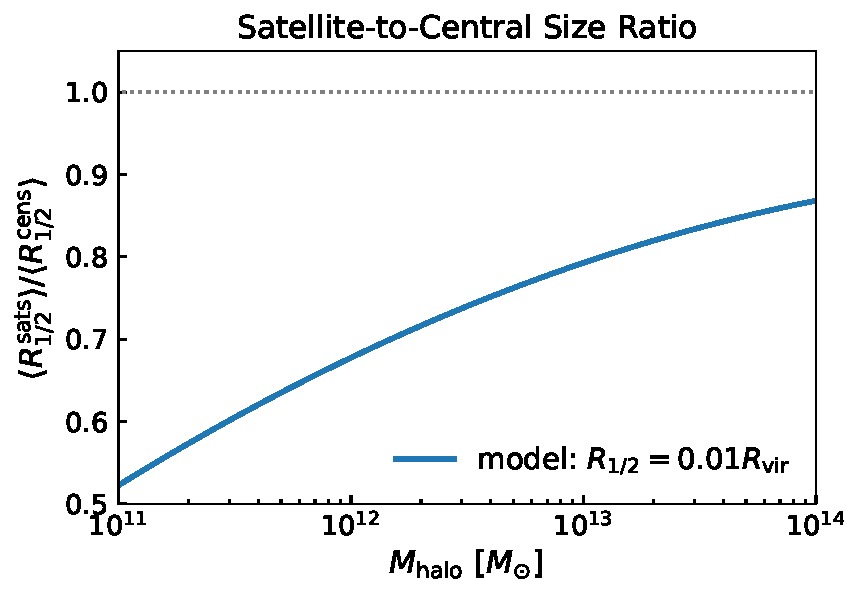
\includegraphics[width=8cm]{FIGS/cen_sat_size_ratios.pdf}
\caption{
{\bf Scaling relation for hydro sims and SAMs.}
As a function of subhalo mass $\mhalo=\mpeak,$ we show the ratio of mean satellite-to-central size predicted by the $\rvir-$based model. This scaling relation should be a useful guideline for more fine-grained physical models of galaxy size that wish to reproduce the observed $\rhalf-$dependence of galaxy clustering.
}
\label{fig:censatsizeratios}
\end{figure}
%-----------------------------------------------------------------------------------------------------

On the one hand, this degeneracy with the satellite fraction is unfortunate, because it means galaxy size does not leave a pure and unique signature on $\rhalf-$clustering ratios. However, this can also be viewed as an opportunity to extract tighter constraints on $F_{\rm sat}(\mstar),$ which are sorely needed to discriminate between competing models \citep{watson_conroy13}. Traditional galaxy clustering is already being used to validate and/or fit models of the stellar-to-halo-mass relation \citep[e.g.,][]{leauthaud_etal11,moster_etal13,behroozi13_smhm,lehmann_etal15}. Based on our results, we advocate that empirical models for $\mean{\mstar}{\mhalo}$ be supplemented with additional model ingredients for $\median{\rhalf}{\mhalo},$ and that the parameters of the composite model be {\em jointly} constrained by measurements of the stellar mass function, $\mstar-$dependent clustering, and $\rhalf-$dependent clustering.

Figure \ref{fig:censatsizeratios} shows that the satellites in $\mhalo\approx10^{12}\msun$ halos can be as large as $\lesssim40-50\%$ smaller than their central galaxy counterparts. Since the satellite fraction varies quite significantly with morphology and/or color, we have demonstrated that it is entirely plausible that most of the observed environmental trends of galaxy size can be understood simply in terms of central vs. satellite size differences. The latter reflects not evolution of galaxies inside host halos, but is due to the fact that satellites have reached their peak mass at higher redshifts than the centrals. While it remains to be seen whether this explanation ends up comprising the whole story, one thing is now clear: it is not possible to reliably analyze environmental trends of galaxy $\rhalf$ without properly accounting for satellites. 

\section{Conclusions}
\label{sec:conclusion}

We have presented new measurements of the dependence of galaxy clustering upon galaxy size, and used {\tt Halotools} to identify the basic ingredients that influence the signal. We conclude with a brief summary of our primary findings:

\ben
\item Small galaxies cluster more strongly than large galaxies of the same stellar mass. Differences between the clustering of small and large galaxies increase on small scales $R\lesssim1\mpc,$ and decrease with stellar mass.
\item The most important ingredient influencing this signal is the relative size of central and satellite galaxies. The magnitude, scale-dependence, and $\mstar-$dependence of $\rhalf-$dependent clustering provides strong evidence that satellite galaxies are smaller than central galaxies of the same halo mass.
\item A simple empirical model in which $\rhalf$ is set by halo $\rvir$ at the time of peak halo mass exhibits a clustering signal that is strikingly similar to that r seen in SDSS.
\item Models in which $\rhalf$ is regulated by $\mstar,$ rather than $\mhalo,$ are grossly discrepant with the observed clustering signal, even when accounting for satellite mass stripping.
\item Taken together, our findings indicate that satellite-specific processes play a sub-dominant role in setting the relative size of centrals and satellites, which instead appears to be largely predetermined at the time of satellite infall.
\een

Our results can be treated as a starting point for more complex and fine-grained models of galaxy size, such as semi-analytic models and hydrodynamical simulations. For convenience, Figure \ref{fig:censatsizeratios} provides a simple summary statistic that can be used as a diagnostic for calibrating alternative modeling efforts. We view the present work as a pilot study that motivates a Bayesian inference program to tightly constrain the galaxy size-halo connection with forward modeling techniques, in direct analogy to the literature on the stellar-to-halo-mass relation. Our publicly available python code provides a simple means for cosmological surveys to generate synthetic galaxy populations with realistic sizes across the cosmic web.

\section*{Acknowledgments}

APH thanks John Baker for the {\em Toejam \& Earl} soundtrack. Thanks also to Frank van den Bosch, Andrew Zentner, Doug Watson, and Risa Wechsler for thoughtful feedback at various stages of the development of this work, and to Faustin Carter and Sebastian Bocquet for sharing their matplotlib expertise.

We thank the {\tt Astropy} developers for the package-template \citep{astropy}, and {\tt NumPy} \citep{numpy_ndarray}, {\tt SciPy} \citep{scipy}, IPython, Matplotlib, and GitHub for their extremely useful free software. While writing this paper we made extensive use of the Astrophysics Data Service (ADS) and {\tt arXiv} preprint repository.

This research was supported in part by the National Science Foundation under Grant No. NSF PHY11-25915. Work done at Argonne National Laboratory was supported under the DOE contract DE-AC02-06CH11357. AK was  supported by NSF grant  AST-1412107 and by the Kavli Institute for Cosmological Physics at the University of Chicago through grant PHY-1125897 and an endowment from the Kavli Foundation and its founder Fred Kavli.

\bibliography{galsize_paper}

\section*{Appendix: Treatment of Disrupted Subhalos}

We use an extension of {\tt Consistent Trees} that models the evolution of subhalos after disruption. The phase space evolution of disrupted subhalos is approximated by following a point mass evolving in the host halo potential according to the orbital parameters of the subhalo at the time of disruption; the evolution of subhalo mass and circular velocity is approximated using the semi-analytic model presented in \citet{jiang_vdB14}. We then use the {\tt orphans} program in {\tt UniverseMachine} to walk through all the Bolshoi-Planck {\tt hlist} files, yielding the main progenitor information of every subhalo that was ever identified by {\tt Consistent Trees}.

Since it is likely that some portion of these disrupted subhalos should be populated with model galaxies \citep{guo_white13, campbell_etal17}, in our initial application of deconvolution abundance matching we derive the $\mstar-\mpeak$ relation using {\em all} subhalos, including those that may be disrupted. We then apply a selection function to the disrupted subhalos, so that a fraction of these objects will host galaxies in our mock universe. We refer to this as the {\em orphan selection function}, $\mathcal{F}_{\rm orphan},$ which we consider to be an integral component of our application of abundance matching.

In this appendix, we show two different, a priori reasonable choices for the orphan selection function. Since a rigorous calibration of $\mathcal{F}_{\rm orphan}$ is beyond the scope of the present work, we instead opt for a simple parameterization that yields reasonably accurate recovery of the galaxy clustering signal observed in SDSS.

In both treatments studied here, we first discard orphan subhalos with $V_{\rm max}/V_{\rm peak}<0.1,$ so that the most drastically disrupted subhalos remain unpopulated with galaxies. For our fiducial model used throughout the main body of the text, $\mathcal{F}_{\rm orphan}$ is defined by randomly selecting half of the orphan subhalos. For the alternative orphan selection function labeled as ``$M_{\rm host}-$dependent orphans" in this appendix, we proceed as follows. We model $\mathcal{F}_{\rm orphan}=\mathcal{F}_{\rm orphan}(M_{\rm peak},M_{\rm host}),$ where $\mpeak$ is the peak mass of the disrupted subhalo, and $\mhost$ is the present-day virial mass of its $z=0$ host halo. For the $\mpeak-$dependence, we select $50\%$ of disrupted subhalos with $\mpeak=10^{11}\msun,$ $0\%$ of subhalos with $\mpeak=10^{13}\msun,$ linearly interpolating in $\log\mpeak$ for intermediate values of $\mpeak.$ At each $\mpeak,$ the selection of disrupted halos is not random; instead, we preferentially select the subhalos with larger $\mhost,$ which we intend to offset the increased difficulty of subhalo-finding algorithms to identify subhalos with especially small values of  $\mu\equiv\mpeak/\mhost.$

Figure \ref{fig:orphan_effects} illustrates the impact of the orphan selection function on $\mstar-$threshold clustering (top panel) and the satellite fraction (bottom panel). Comparing the black to the red curves shows that including orphans substantially boosts small-scale clustering due to the increased satellite fraction. Comparing the orange to the black curves, we see that random orphan selection, vs. the $M_{\rm host}-$dependent selection, results in similar clustering, with slight differences on the smallest scales at the highest masses. Because we have not been systematic in the calibration of $\mathcal{F}_{\rm orphan},$ we adopt the simpler, random orphan selection as the fiducial model shown in the main body of the text.

%---------------------------------------------------------------------------------------------------
\begin{figure}
\centering
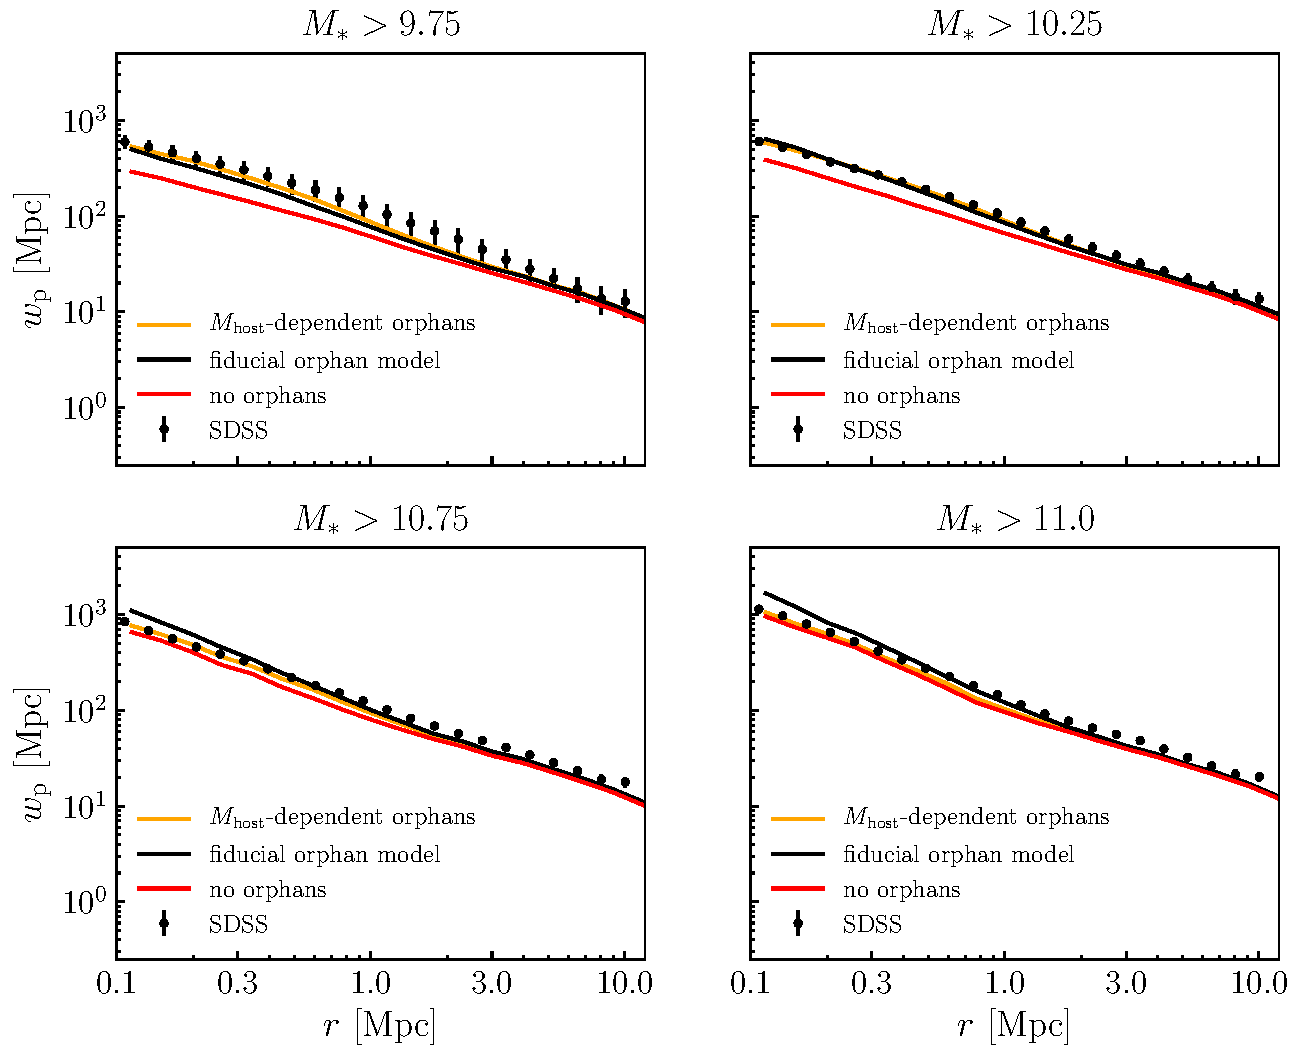
\includegraphics[width=8cm]{FIGS/baseline_sham_orphans.pdf}
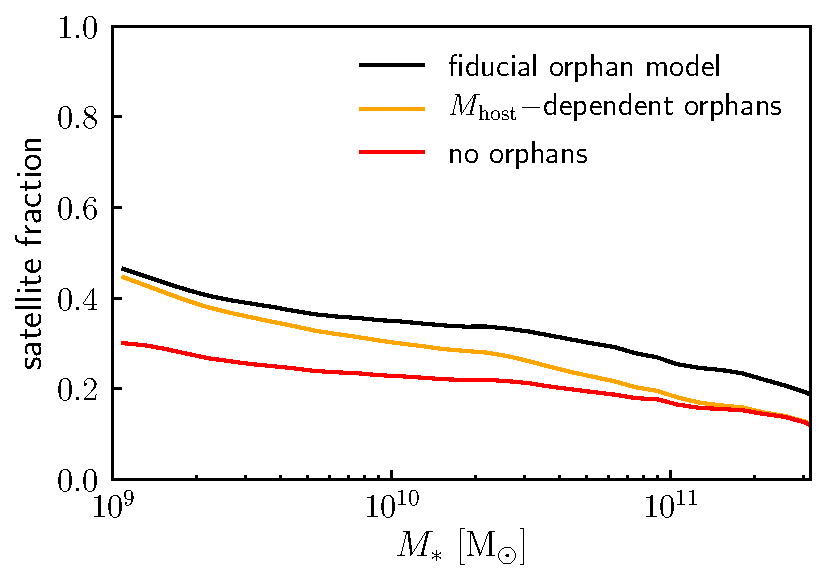
\includegraphics[width=8cm]{FIGS/orphan_satellite_fraction.pdf}
\caption{
{\bf Impact of the orphan selection function.} The {\em top panel} is identical to Figure \ref{fig:baseline_sham_clustering}, but includes additional curves for the case of $M_{\rm host}-$dependent orphan selection (orange curves), and no orphans at all (red curves). As a function of stellar mass, the {\em bottom panel} shows the satellite fraction, i.e., the fraction of objects that are not central galaxies.
}
\label{fig:orphan_effects}
\end{figure}
%-----------------------------------------------------------------------------------------------------

\end{document}







